\documentclass{article}
\usepackage{amsmath, amsthm, amssymb, amsfonts}
\usepackage{thmtools}
\usepackage{graphicx}
\usepackage{setspace}
\usepackage{geometry}
\usepackage{float}\usepackage{hyperref}
\usepackage[utf8]{inputenc}
\usepackage[english]{babel}
\usepackage{framed}
\usepackage[dvipsnames]{xcolor}
\usepackage{tcolorbox}
\usepackage{outlines}
\newcounter{Chapcounter}


\newcommand\showmycounter{\addtocounter{Chapcounter}{1}\themycounter}
\newcommand{\chapter}[1] 
{ {\centering          
  \addtocounter{Chapcounter}{1} \Large \underline{\textbf{ \color{blue} Chapter \theChapcounter: ~#1}} }   
  \addcontentsline{toc}{section}{ \color{blue} Chapter:~\theChapcounter~~ #1}    
}

\colorlet{LightGray}{White!90!Periwinkle}
\colorlet{LightOrange}{Orange!15}
\colorlet{LightGreen}{Green!15}
\colorlet{LightLavender}{Lavender!15}
\newcommand{\HRule}[1]{\rule{\linewidth}{#1}}

\declaretheoremstyle[name=Theorem,]{thmsty}
\declaretheorem[style=thmsty,numberwithin=section]{theorem}
\tcolorboxenvironment{theorem}{colback=LightGray}

\declaretheoremstyle[name=Proposition,]{prosty}
\declaretheorem[style=prosty,numberlike=theorem]{proposition}
\tcolorboxenvironment{proposition}{colback=LightOrange}

\declaretheoremstyle[name=Principle,]{prcpsty}
\declaretheorem[style=prcpsty,numberlike=theorem]{principle}
\tcolorboxenvironment{principle}{colback=LightGreen}

\declaretheoremstyle[name=Example,]{exsty}
\declaretheorem[style=exsty,numberlike=theorem]{example}
\declaretheoremstyle[name=Definition,]{defsty}
\declaretheorem[style=defsty,numberlike=theorem]{definition}
\setstretch{1.2}
\geometry{
    textheight=9in,
    textwidth=5.5in,
    top=1in,
    headheight=12pt,
    headsep=25pt,
    footskip=30pt
}

% ------------------------------------------------------------------------------

\begin{document}

% ------------------------------------------------------------------------------
% Cover Page and ToC
% ------------------------------------------------------------------------------

\title{ \normalsize \textsc{}
		\\ [2.0cm]
		\HRule{1.5pt} \\
		\LARGE \textbf{\uppercase{STA 237 Notes} \vspace*{10\baselineskip}}
		}
\date{}
\author{\textbf{Author} \\ 
		Hao Hua He \\}

\maketitle
\newpage

\tableofcontents
\newpage

% -----------
\chapter{Week 1}
\section{Lec 1: Outcomes, Events. and Probability}
\subsection{Introduction}
Definitions
\begin{outline}[enumerate]
\1 \textbf{Probability}
\2 numeric value of certainty/uncertainty
\1 \textbf{(Random) Experiment}
\2 mechanism/phenomenon that results in random or unpredictable outcomes
\1 \textbf{Sample Space}
\2 Set of all outcomes from an experiment
\2 denoted $\Omega$
\1 \textbf{Event}
\2 Subset of Sample Space
\2 \underline{Relations between events}
\3 INtersect
\3 Union
\3 Complement
\end{outline}

\begin{example}
Neither $A$ not $B$ is denoted $(A\cup B)^c \Rightarrow A^c \cap B^c$
\end{example}
\begin{theorem}
\textbf{De Morgan's Law} sates for any events $A$ and $B$
\begin{outline}[enumerate]
\1 $(A \cup B)^c = A^c \cap B^c$
\1 $(A \cap B)^c = A^c \cup B^c$
\end{outline}
\end{theorem}
\begin{example}
Exactly one of $A$ and $B$ is denoted as $$A\cup B \cap (A \cup B)^c = A \cup B \cap (A^c \cup B^c)$$
\end{example}
More Definitions:
\begin{outline}[enumerate]
\1 \textbf{Disjoint(mutually exclusive)}
\2 $A\cap B = {} = \varnothing$
\1 $A$ implies $B$
\2 $A \subset B$
\2 $A \cap B = A$
\end{outline}
\newpage
%------------------------------------------------
\subsection{Probability Function}
\subsubsection{Definition}
\begin{definition}
Probability func $P$ defined on a \underline{finite} sample space $\Omega$ assigns each event $A \in \Omega$ a number $P(A)$ s.t.
\begin{outline}[enumerate]
\1 $P(A)\geq 0$
\1 $P(\Omega) = 1$
\1 $P(A \cup B) = P(A) + P(B)$
\2 if $A$ and $B$ disjoint.
\end{outline}
where $P(A)$ is the probability that event $A$ occurs.
\end{definition}
\subsubsection{Calculating by Counting}
Calculating by counting only applies when
\begin{outline}[enumerate]
\1 All outcomes of $\Omega$ are equally likely
\2 $\Omega$ is finite
\end{outline}
Then,
$$P(A) = \frac{\text{number of outcomes belonging to } A}{\text{ Total number of outcomes in }\Omega}$$
%\begin{theorem}
%    This is a theorem.
%\end{theorem}
%
%\begin{proposition}
%    This is a proposition.
%\end{proposition}

%\begin{principle}
%    This is a principle.
%\end{principle}

% Maybe I need to add one more part: Examples.
% Set style and colour later.
\subsubsection{Product of sample space}
In general, given sample spaces $\Omega_1$ and $\Omega_2$, we have $$\Omega = \omega_1 \times \omega_2 = \{(\omega_1, \omega_2): \omega_1 \in \Omega_1, \omega_2 \in \Omega_2)\}$$
\subsubsection{Permutation and Combination}
Permutations and combinations are ways of grouping elements of a set into a subset, where permutations are ordered and combinations are unordered.
\begin{theorem}
The number of possible permutations of size \emph{n} from \emph{N} objects
$$_NP_n = \frac{N!}{(N-n)!}$$
\end{theorem}
\begin{theorem}
The number of possible combinations of size \emph{n} from \emph{N} objects
$${N \choose n} = \frac{N!}{(N-n)!}$$
\end{theorem}
\newpage
\section{Lec 2: Conditional Probability and Independence}
\subsection{Conditional Probability}
Conditional probability of an event \emph{A} given event \emph{C} is, for any $C$ with $P(C) > 0$,
$$P(A|C) = \frac{P(A\cap C)}{P(C)}$$
or alternatively, with the multiplication rule
$$P(A\cap C) = P(A|C) \cdot P(C)$$
\subsubsection{Law of Total Probability}
Suppose events $C_1, \dots, C_2$ are disjoint s.t. $C\cup \dots \cup C_m = \Omega$, for any arbitrary $A$,
$$P(A) = \sum^m_{i=1}[P(A|C_i)P(C_i)]$$
Thus,
\begin{align*}
P(C_i|A) &= \frac{P(C_i)\cap A}{P(A)}\\
&= \frac{P(A|C_i)P(C_i)}{\sum^m_{i=1}[P(A|C_i) P(C_i)]}
\end{align*}
\subsubsection{Baye's Rule}
Suppose $C_1, \dots, C_m$ are disjoing s.t. $C\cup \dots \cup C_m = \Omega$, the conditional probability of $C_i$ given any arbitrary $A$ is
$$P(C_i|A)=\frac{P(A|C_i)\cdot P(C_i)}{\sum^m_{i=1}[P(A|C_i)P(C_i)]}$$
\newpage
\subsection{Independence}
\subsubsection{Definition}
\begin{definition}
Events $A$ and $B$ are independent if
$$P(A|B) = P(A)$$
That is to say that $B$ occuring or not does not change the probability of $A$
\end{definition}
\hbox{}
\subsubsection{Implications}
\begin{outline}[enumerate]
\1 Suppose $A$ and $B$ with $P(A|B) = P(A)$
\2 Complements
\3 $P(A^c|B) = P(A^c)$
\2 Mulplication Rule
\3 $P(A\cap B) = P(A)P(B)$
\2 Mutal Property
\3 $P(B|A) = P(B)$
\end{outline}
To show that $A$ and $B$ are independent, one of the following must be proved, otherwise $A$ and $B$ are dependent.
\begin{align*}
P(A^c|B) = P(A^c) &\iff\\
P(A\cap B) = P(A)P(B) &\iff\\
P(A|B) = P(B)&
\end{align*}
\newpage
\chapter{Week 2}
\section{Lec 3: Discrete Random Variables}
\subsection{Discrete Random Variables}
\par Let $\Omega$ be a sample space. A \textbf{random variable} $X$ is a function that maps $\Omega$ on to a real number ($\mathbb{R}$)
\begin{definition}
When a \emph{random variable} $X$ takes a countable number of values, it is called a \textbf{discrete random variable} 
\end{definition}

\subsection{Probability mass function}
\begin{definition}
The \textbf{probability mass function} $p$ of a discrete random variable $X$ is the finction
$$p:\mathbb{R} \to [0,1]$$
defined by
\begin{align*}
&p(k) = P(X=k)\\
\text{for } &-\infty < k < \infty
\end{align*}
\end{definition}
The probability mass function \textbf{uniquely} defines the behaviour of a random variable.
\subsection{Cumulative distribution function}
\begin{definition}
The \textbf{cumulative distrubution function}, or \textbf{distribution function} $F$ of a random variable $X$ is the function
$$F: \mathbb{R} \to [0,1]$$
defined by
\begin{align*}
&F(A) = P(X\leq a)\\
\text{for }& -\infty < a < \infty
\end{align*}
\end{definition}
\subsection{Bernoulli distribution}
A disc
\newpage
\section{Lec 4: Continuous Random Variables}
\begin{definition}
A random variable $X$ is \textbf{continuous} if for some function
$$f: \mathbb{R} \to \mathbb{R}$$
and any numbers $a$ and $b$ with $a\leq b$,
$$P(a\leq X \leq b) = \int^b_a f(x) dx$$.
Note: the function has to satisfy
\begin{outline}[enumerate]
\1 $f(x) \geq 0$ for all $x$ and
\1 $\int^\infty_{-\infty} f(x)dx = 1$
\end{outline}
We call this function $f$ the \textbf{probability density fuction} of $X$ and the value(s) of $f(x)$ is the \textbf{probability density} of $X$ at $x$
\end{definition}
\begin{outline}[enumerate]
\1 $f(x)$ is \textbf{not} probability
\1 Both a pmf and pdf uniquely defines a random variable, but a pmf maps to $[0,1]$ and a pdf to $[0,1)$
\1 $f(x)$ can be interpreted as a relative measure of likelihood around $X$
\end{outline}
\begin{definition}
The \textbf{cumulative distrubution function of} $F$ of a random variable $X$ is the function
$$F: \mathbb{R} \to [0,1]$$
defined by
\begin{align*}
&F(x) = P(X\leq a)\\
\textbf{for } &-\infty < a < \infty
\end{align*}
Note: the definition of \emph{cdf} is the same for both discrete and continuous random variables	
\end{definition}
\subsection{Property of cumulative distribution functions}
\begin{center}
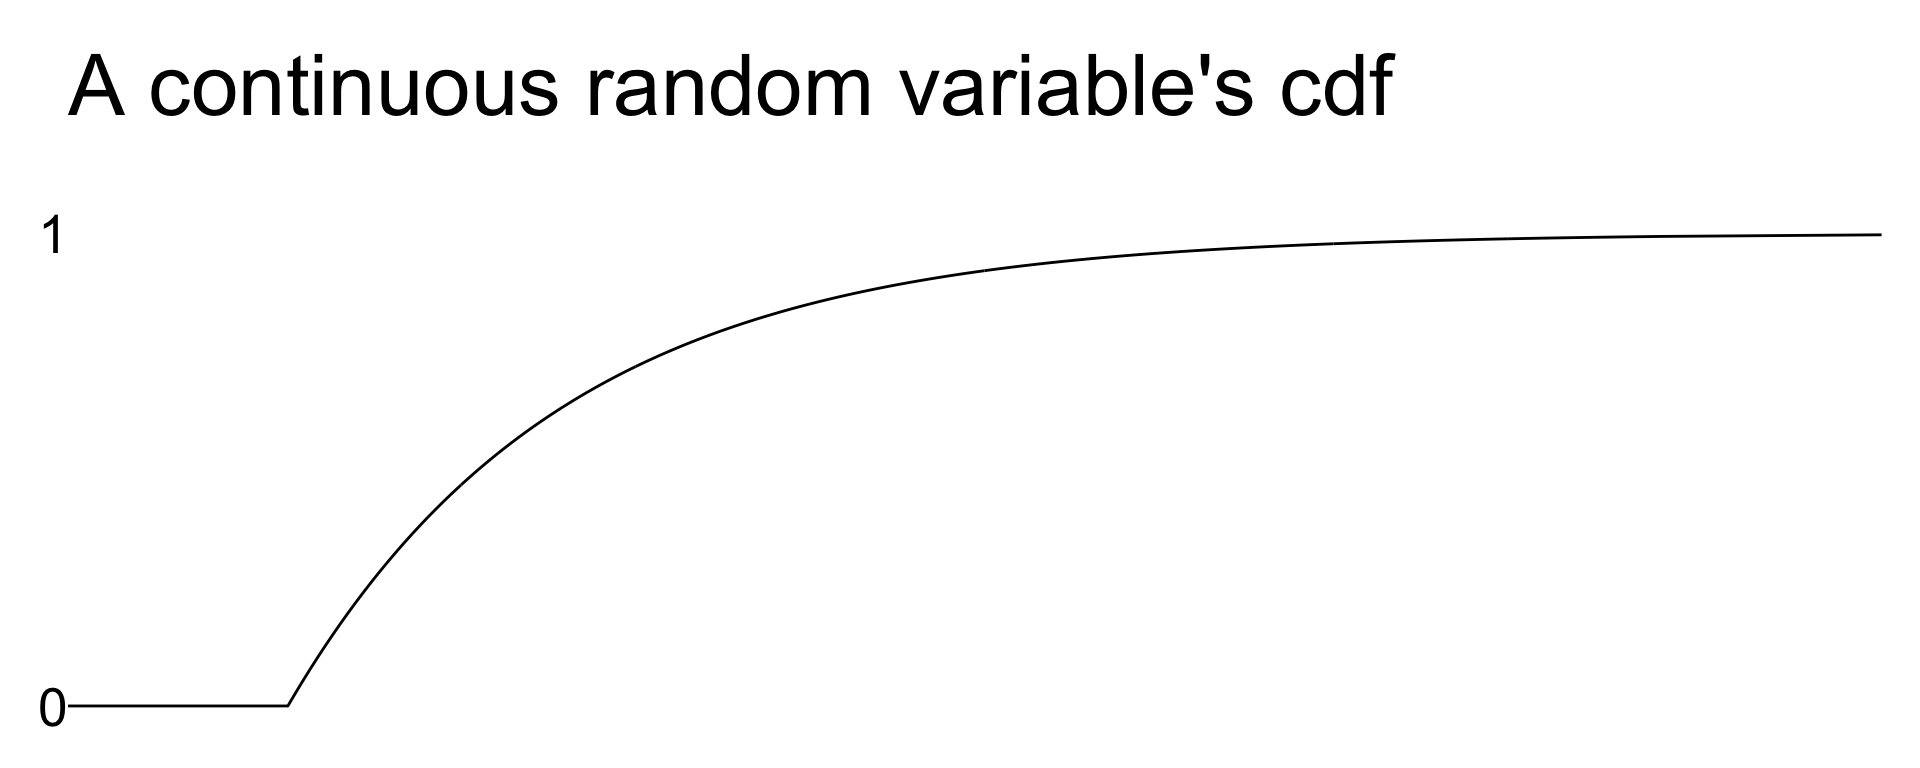
\includegraphics[scale=.15]{crvcdf.png}
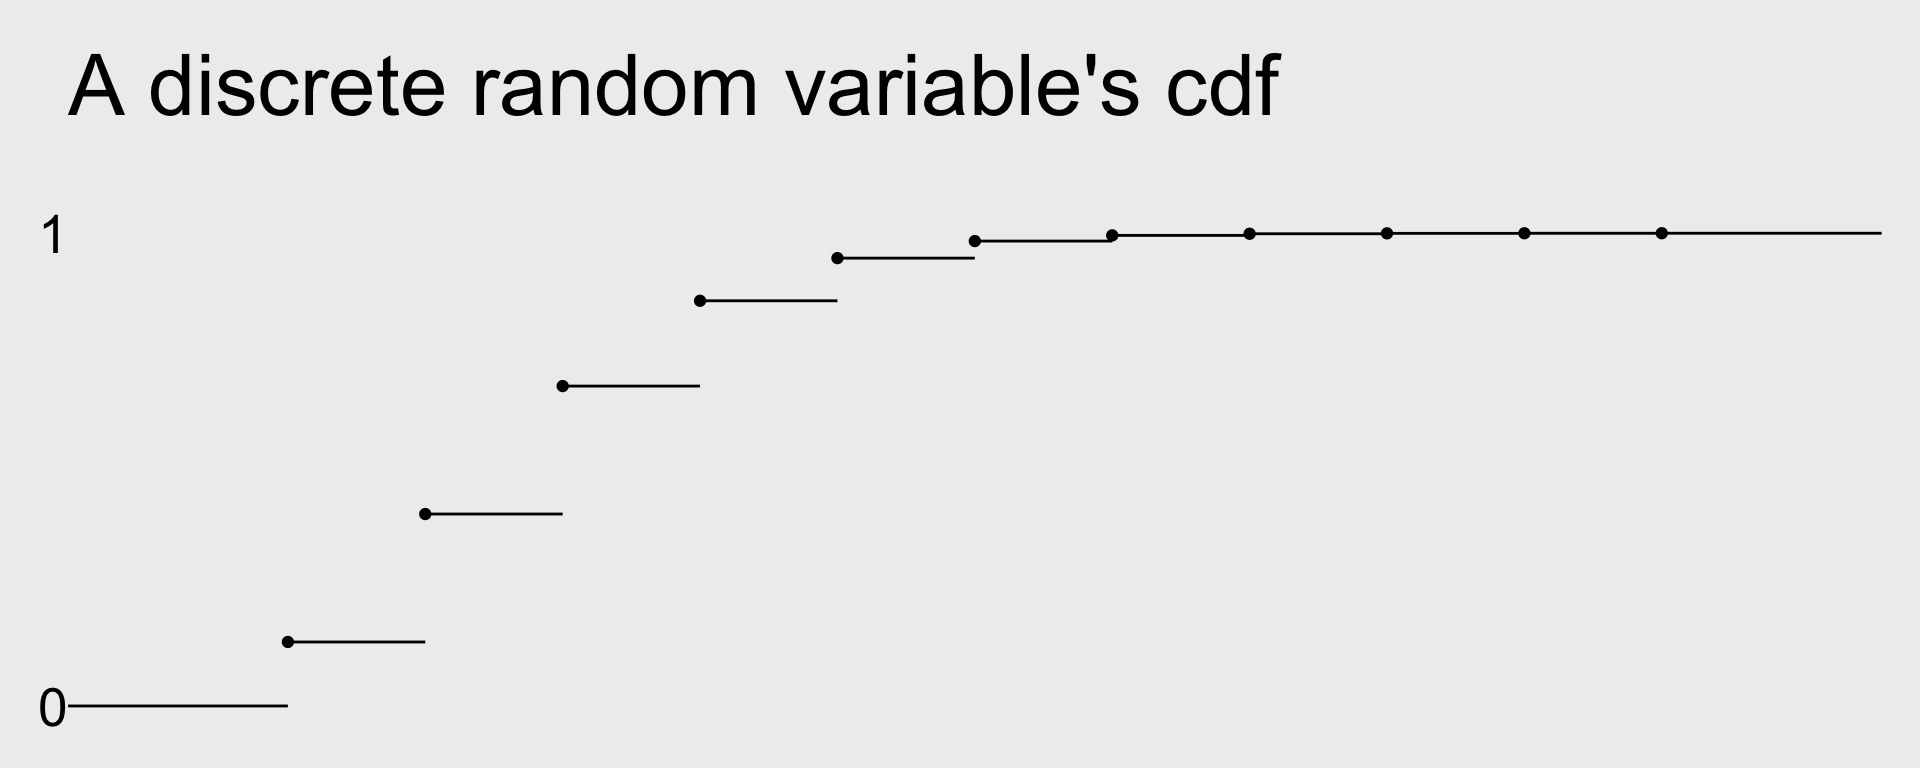
\includegraphics[scale=.15]{drvcdf.png}
\end{center}
\par Any cdfs are
\begin{outline}[enumerate]
\1 Non-decreasing
\1 Right continuous and
\1 (Approaching) 0 on the left end and to 1 on the right end
\end{outline}
\subsection{Quantile, Percentile, and Median}
\begin{definition}
Let $X$ be a random variable with cumulative distribution function $F$. Then the \textbf{quantile funtion} of $X$ is the function $F^{-1}$ defined by
$$F^{-1}(t) = \min(x: F(x) \geq t)$$
for $0 < t < 1$
\end{definition}
\subsubsection{Quantile function for continuous vs discrete}
\begin{center}
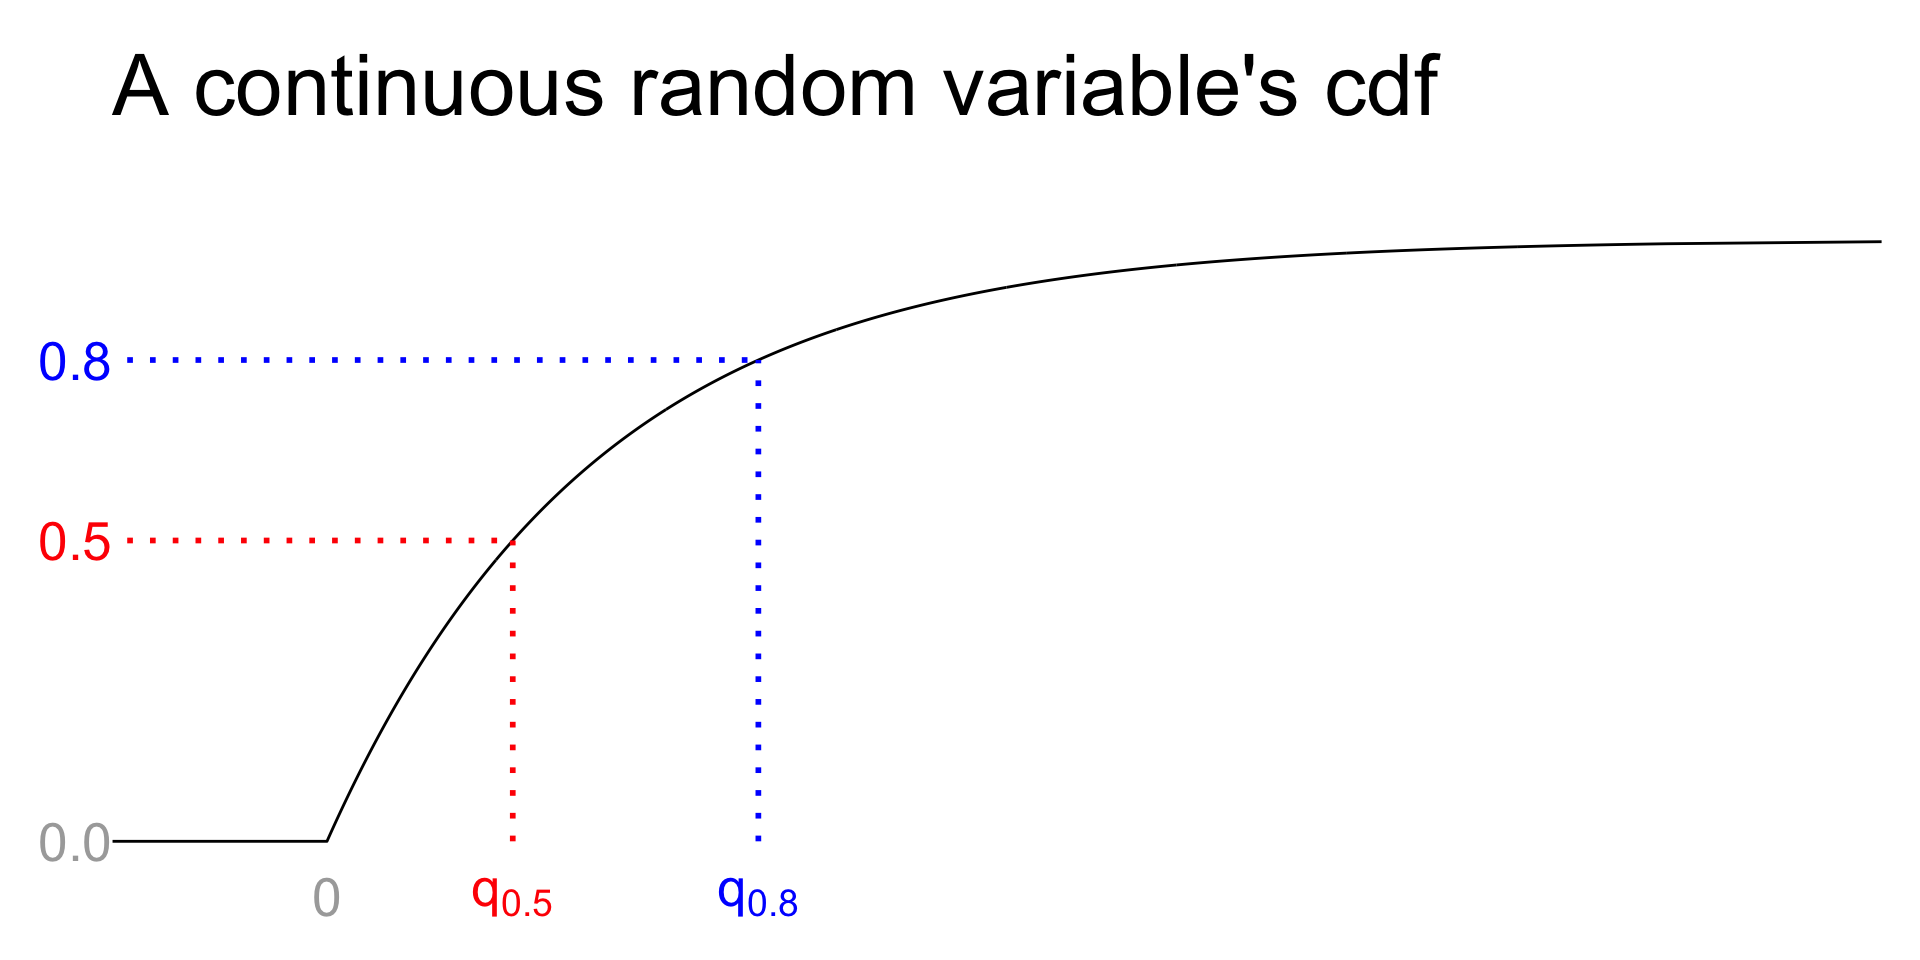
\includegraphics[scale=.15]{crvqf.png}
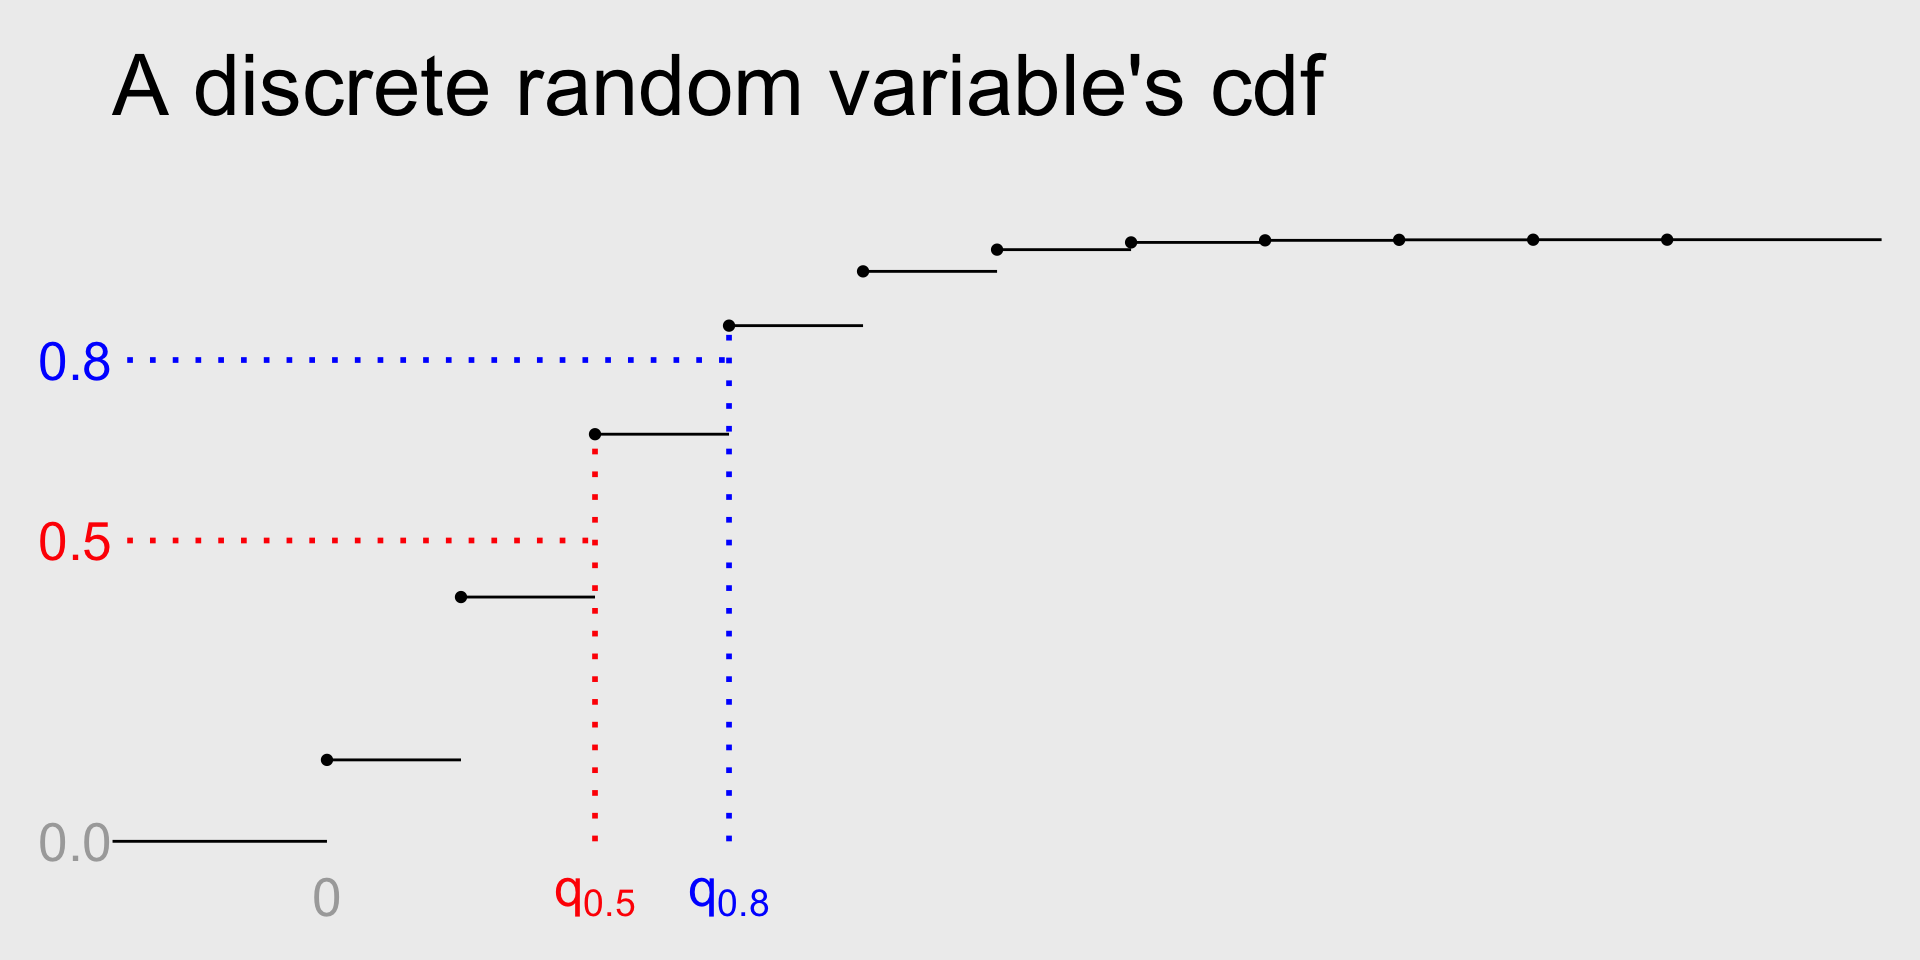
\includegraphics[scale=.15]{drvqf.png}
\end{center}
\subsection{Common Continuous Distributions}
\subsubsection{Uniform distribution}
\begin{definition}
A continuous random variable has a \textbf{unitiorm distribution} on interval $[\alpha, \beta]$ if its probability density funtion $f$ is given by\\
\begin{equation}
f(x) =
\begin{cases}
\frac{1}{\beta -\alpha} \ \ &\alpha \leq x \leq \beta\\
0 \ \ &otherwise
\end{cases}
\end{equation}
\end{definition}
\subsubsection{Exponential Distribution}
\begin{definition}
A continuous random variable has an \textbf{exponential distribution} with parameter $\lambda, \lambda > 0$ if its probability density function $f$ is given by\\
\begin{equation}
f(x) =
\begin{cases}
\lambda e^{-\lambda x} \ \ &x \geq 0\\
0 \ \ &otherwise
\end{cases}
\end{equation}
Exponential random variables are often used to model time until the next event in a Poisson process. $\lambda$ is the expected rate of events.
\end{definition}
\textbf{Memoryless Property of Exponential Random Variables}
\subsubsection{Gamma Distribution}
\begin{definition}
A continuous random variable has a \textbf{gamma distribution} with parameyers $\alpha$ and $\beta$ with $\alpha > 0$ and $\beta > 0 $ it its propability density $f$ is given by
\begin{equation}
f(x) = \frac{1}{\Gamma(\alpha)} \beta^\alpha x^{\alpha -1} e^{-\lambda x} \ \ \text{for $x > 0$}
\end{equation}
We denote this distrubution Gamma$(\alpha, \beta)$
\end{definition}
\subsubsection{Normal Distribution}
\begin{definition}
A continuous random variable has a \textbf{normal distribution} with parameter $\mu$ and $\sigma^2$ with $\sigma^2 > 0$ it its probability density function $f$ is given by
\begin{equation}
f(x) = \frac{1}{\sigma \sqrt{2\pi}}\exp\{-\frac{1}{2}(\frac{x-\mu}{\sigma})^2\}
\end{equation}
\end{definition}
\par Normal distribution, or Gaussian distribution, ins central in probability theory and statistics.\\
\par It is often used to model observational errors.\\
\par Normal distributions have a symettric shape around its centre.\\
\par $\mu$ controls the center of the distribution (location) while the $\sigma$ controls the spread of the distribution (shape)\\

\begin{definition}
A normal distribution with $\mu = 0$ and $\sigma^2 = 1$ is called the \textbf{standard normal distribution}.\\

We often denote a srandard normal random variable by $Z$, $Z ~ N(0,1)$ is its pdf with $\phi$, and its cdf with $\Phi$
\end{definition}
\chapter{Week3}
\section{Lec 5: Expectation and Variance}
\subsection{Expectation}
\subsubsection{Expectration of DRV}
\begin{definition}
The expectation of  DRV $X$ taking values $x_1,\dots,x_2$ with probability mass function $p$ is given by  $$E[X] = \sum_{i\in\{1,2,\dots\}}x_i p(x_i)$$
\end{definition}

\subsubsection{Expectation of CRV}
\begin{definition}
The \textbf{Expectation} of a CRV $X$ with pdf $f$ is given by $$E[X] = \int^\infty_{-\infty}xf(x)dx$$
\end{definition}
\subsection{Variance}
\begin{definition}
The \textbf{Variance} of a random variable $X$ is the number defined by $$\text{Var}(X)x	 = E[(X-E[X])^2]$$
\end{definition}

%-------------------------
\newpage
\chapter{Summation of Definitions and theorems}
\section{Definitions}
\begin{outline}[enumerate]
\1 \textbf{Event}
\2 Subset of Sample Space
\2 Relation between events
\3 Intersect
\4 denoted $A \cap B$
\3 Union
\4 denoted $A \cup B$
\3 Complement
\4 denoted $A^c$
\1 \textbf{Event}
\2 Subset of sample space
\1 \textbf{(Random) Experiment}
\2 Mechanism/Phenomenon that results in random or unpredictable outcomes
\1 \textbf{Probability}
\2 Numeric  Value of certainty/uncertainty
\1 \textbf{Sample Space}
\2 Set of all possible outcomes (from experiment)
\2 Denoted $\Omega$
\end{outline}
\section{Theorems}
% ------------------------------------------------------------------------------
% Reference and Cited Works
% ------------------------------------------------------------------------------

\bibliographystyle{IEEEtran}
\bibliography{References.bib}

% ------------------------------------------------------------------------------

\end{document}
